\chapter{General discussion}
\label{sec:conclusion}

\section{Research findings in context}
``EEG is a record of the oscillations of brain electric potential.'' So begins the book \textit{Electric fields of the brain: the neurophysics of EEG} by Nunez and Srinivasan \cite{Nunez2006}, the most widely cited reference for EEG theory. Perhaps EEG is a record of more.

Of all the conclusions from this thesis, the strongest and best supported is the conclusion that broadband EEG features reflect synaptic physiology --- and this physiology is not necessarily static. It has been long established that EEG signals reflect synaptic currents (\autoref{sec:standard_model}) and several papers have built upon the idea that the spectral trend reflects a stochastic processes filtered by synaptic kinetics (\autoref{sec:timescales}). Many of the important gaps in this theory were filled by the modelling results of \autoref{sec:natcomms}, thus strengthening the theoretical foundation of this hypothesis. Moreover, \autoref{sec:apEEG} demonstrated that synaptic timescales are alone sufficient to explain the neural origins of the spectral trend in EEG. Finally, the experiments in  \autoref{sec:natcomms} showed that pharmacologically altering synaptic timescales caused differences in the spectral trend that exactly matched theoretical predictions, providing the first experimental validation of the synaptic timescale hypothesis. In fact, most of the theories on the spectral trend have tried to explain its default scaling behaviour, which as discussed in \autoref{sec:intro} can be explained in many distinct ways. To the best of our knowledge, our results provide the first experimental validation of any of the theories on the spectral trend. Not all of the theories on the spectral trend are mutually exclusive, however, and the results of this thesis have important implications for all of them.

\subsubsection{Local versus global synchrony: the classical view}
Our results illustrate that synaptic timescales will filter all synaptically generated EEG signals. Therefore, even under the classical view that the EEG signal is a superposition of brain rhythms, the resulting EEG oscillations will still be filtered by synaptic kinetics, with the consequence that faster oscillations will be attenuated compared to slower oscillations. In other words, slower oscillations need not be more widely synchronized than faster oscillations to generate the $1/f$ trend. Given the current evidence, it is possible that slow oscillations tend to be more globally synchronized; however, the argument made by Buszaki and colleagues is that this correlation specifically produces a power law \cite{Buzsaki2006,Penttonen2003}. With the addition of synaptic timescales as an alternate explanation for the power-law, the validity of the all-brain-rhythms viewpoint is not necessarily conditional on the validity of this foregoing assertion. Therefore, considering the inconsistent evidence for the power-law relationship among brain rhythms (\autoref{sec:all_oscillations}), the results of this thesis strengthen the standing of the theory that EEG signals only reflect brain rhythms. 

\subsubsection{Self-organized criticality}
Despite the foregoing discussion, our results also provide some evidence in support of the self-organized criticality theory. Whereas neural synchrony is typically associated with oscillations, our results demonstrate that a network obeying the dynamics of a branching process can generate synchronized dipoles as the processes approaches criticality. We found that even subcritical dynamics consistent with experimental measurements \cite{Wilting2018,Wilting2019,Suryadi2022} produce sufficient levels of synchronized neural activity, meaning that oscillations are not required for generating detectable EEG signals. Our results therefore validate that the EEG spectral trend could theoretically reflect aperiodic neural activity. However, whether it does in practice remains to be established. Demonstrating this experimentally could be possible if a preparation could be designed where, for example, the failure rate of synaptic transmission is increased to bring down the effective branching number in neural networks. While it would be difficult to manipulate network criticality without affecting brain rhythms, such experiments could provide supporting evidence for this theory especially when coupled with quantitative, theoretical predictions.

\subsubsection{Tissue filtering}
Consistent with the idea that neural tissue conductivity is minimally frequency dependent, the timescale of synaptic currents were alone sufficient to capture the scaling of EEG signals. The tissue filtering idea was used by Bedard et al. \cite{Bedard2006a} to explain the extra $1/f$ factor observed in their LFP spectra. An understated result of \autoref{sec:natcomms} is that, while exponentially decaying synaptic currents indeed can only generate scaling with an exponent of $\beta=2$, once more realistic kinetics were considered by including a rise and decay time constant, synaptic timescales actually produced an asymptotic scaling of $\beta=4$, exactly that seen by Miller et al \cite{Miller2009}! Indeed, synaptic currents alone can explain spectral exponents from 0 to 4 depending on the interplay between the synaptic contributions to the signal, the high frequency plateau, and the frequency range over which the exponent is measured.

\subsubsection{Dendritic filtering}
Our results suggest that synaptic kinetics alone are sufficient to explain the scaling in EEG spectra. So what of the effects of dendritic filtering? An important distinction between our simulations and those by Pettersen et al. \cite{Pettersen2014} is that these authors injected white noise into the dendrites of their neuron models, whereas we simulated actual synaptic inputs. In essence, our inclusion of the rise and decay times of synaptic currents (\ref{eq:fitting}) already incorporates the aspects of dendritic filtering theory \cite{Linden2010, Pettersen2008, Pettersen2014}. This is because we constrained the kinetics of synapses based on in vitro recordings of postsynaptic currents which were measured in the soma~\footnote[2]{Indeed, it is almost impossible to measure the kinetics of synaptic currents at the location of the synapse on the dendrite, although the refinement of fluorescence voltage indicators is making this a reality \cite{Knopfel2019}.}. Therefore, our parameters implicitly include the low-pass filtering effects of the dendrites. As shown in \autoref{fig:figure2.1}d, the spectrum of the electric potential generated far away from the single-neuron can be entirely explained by synaptic kinetics, although notably the measured timescale from the spectrum is slightly slower than the kinetics of the synaptic conductances used in the model (\autoref{fig:figure2.1}e). This difference is the fingerprint of dendritic filtering in our simulations. 

\subsubsection{High frequency plateau}
Finally, with respect to theories on the high frequency plateau observed in macroscopic neural recordings, the results in \autoref{sec:apEEG} provide strong theoretical evidence to reject the idea that the high frequency plateau in EEG signals reflects broadband spiking activity. However, our results indicate that above $\sim$\qty{100}{\hertz}, the contributions of synaptic currents decay below the noise floor of the amplifier, meaning everything above this threshold is likely not synaptic in origin. Our results suggest that action potentials, instead of synaptic currents, generate EEG rhythms in this frequency range. Consequently, a broadly tuned high gamma oscillations could generate EEG signals from action potentials that appear broadband in nature depending on the time window over which the spectrum is computed and the frequency range over which the spectrum is analyzed. Therefore, the implication of our findings for the high frequency plateau may depend on how this feature is operationally defined.

\section{Extended discussion points}

\subsection{Neural basis of EEG}
Our modelling outcomes and experiments suggest that EEG spectra are strongly shaped by inhibitory timescales. However, this view contrasts with past studies that have modelled both periodic and aperiodic EEG signals exclusively as the sum of excitatory synaptic currents \cite{Miller2007,Jensen2005,McCarthy2008,Ching2010}. One possible explanation for this divergence is that inhibition is often considered to be mainly perisomatic, where input necessarily elicits dipoles of low amplitude \cite{Nunez2006,Næss2021,Ahlfors2015}. In our model, inhibitory synapses were formed throughout the dendritic trees including the apical tufts of pyramidal cells, in line with anatomical and electrophysiological studies \cite{Palmer2012, Karimi2020, Iacaruso2017}. While both excitation and inhibition contributed with similar magnitudes to single-neuron dipoles, the slow kinetics of GABA\textsubscript{A} receptors caused inhibition to dominate low frequency power.

Our biophysical calculations indicated that almost the entire amplitude of aperiodic EEG signals results from dipole synchrony. Differences in synchrony between excitatory and inhibitory inputs across neurons may therefore play a larger role in shaping the EEG spectrum than excitation/inhibition balance at the membrane level. Indeed, in vivo recordings of spontaneous activity suggest that inhibitory neurons spontaneously fire more synchronously than excitatory neurons \cite{Gentet2010}; this alone could explain the stronger contributions of inhibitory currents to the EEG. In a similar vein, our results from \autoref{sec:apEEG} suggest that action potentials from both excitatory and inhibitory neurons contribute to high frequency scalp potentials. Thus, several lines of evidence throughout our work converge on the idea that inhibitory neurons and inhibitory synaptic currents contribute significantly to the EEG signal. This idea suggests that it is an oversimplification to consider excitatory synapses and pyramidal neurons as the sole sources of EEG signals (\autoref{sec:standard_model}).

\subsection{Consciousness and anesthesia} \label{sec:anesthesia}
LFP recordings in humans have demonstrated that loss of consciousness from propofol is accompanied within seconds by a sudden increase in delta rhythms \cite{Lewis2012}. Interestingly, when analyzing baseline-normalized spectra, our EEG recordings suggested that delta power increased well before loss of consciousness (\autoref{fig:figure2.9}); only after detrending our EEG spectra were our measurements consistent with this past study. The fact that propofol did not seemingly distort the time course of delta rhythms in the LFP study \cite{Lewis2012} could suggest that the relative contribution of inhibitory and excitatory currents to LFP differs from EEG, with LFP recordings predominantly shaped by excitatory currents. This could make sense if inhibitory currents are more synchronized than excitatory currents, as discussed in the previous section, because EEG reflects larger volumes of tissue and is therefore more strongly biased by widespread synchrony than LFP. This possibility should be explored further to tie together theories of the spectral trend across recording modalities. 

Propofol's mechanism of action has been significantly elucidated in the last two decades. Its suppression of breathing, eye reflexes, and muscle tone are all thought to result directly from GABAergic inhibition of various brain stem areas \cite{Brown2011}. Propofol is thought to induce unconsciousness through the inhibition of arousal centers in the brain stem as well as a potentiation of thalamic reticular neurons and cortical interneurons \cite{Brown2011}. Notably, in sleep, delta rhythms are thought to result from thalamic neurons switching from spiking to bursting upon a drop in excitatory cholinergic input from the brain stem (\autoref{sec:delta}). The suppression of cholinergic neurons in the laterodorsal and pedunculopontine tegmental areas by propofol \cite{Brown2011} would suggest that propofol causes its delta rhythms in a similar manner. The sharp binary switch in delta rhythm amplitude observed here (\autoref{fig:figure2.9}) would be consistent with a sudden bifurcation in thalamic firing pattern. 

However, this interpretation contrasts with the idea that the propofol delta rhythm is generated intracortically, unlike the sleep delta rhythms \cite{Akeju2017d}. This interpretation is based on two arguments. First, unlike the sleep delta rhythm, propofol delta is fragmented and not synchronized over large areas \cite{Akeju2017d,Lewis2012}. Second, delta amplitude increases in a dose dependent manner until reaching a plateau \cite{Akeju2017d,NiMhuircheartaigh2013}. This latter observation was interpreted as a steady increase in the number of cortical neurons oscillating synchronously \cite{NiMhuircheartaigh2013}, which is inconsistent with the ``thalamic switch'' hypothesis. Our results propose an alternate interpretation, namely that the dose-dependent increase in low frequency power was the direct result of a dose-dependent slowing of inhibitory synaptic kinetics (\autoref{fig:figure2.8}). To the first argument, complete reconstruction of thalamocortical neuron morphologies in mice indicate axon termination fields that span almost \qty{1}{\milli\meter} \cite{Winnubst2019}. It is therefore possible that the fragmented delta rhythms observed in propofol anesthesia are generated by delta-bursting thalamocortical neurons that are simply not synchronized with each other, thus producing delta oscillations that are only synchronized over a couple millimeters. In summary, our study provides some evidence for the thalamic switch hypothesis, but further investigations are still needed.

Finally, Ni Mhuircheartaigh et al. \cite{NiMhuircheartaigh2013} argued that the dose-dependent increase in delta oscillations could potentially be used to help titrate optimal propofol dosage in the operating room. Our results strongly support this idea and moreover suggest it could be possible to actually determine the effect-site concentration empirically using the extracted inhibitory synaptic timescales from the EEG spectrum. While the experiments performed in \autoref{sec:natcomms} used a fast induction of loss of consciousness, propofol can also be administrated using a target effect-site concentration protocol, where propofol is administrated to maintain a constant, predetermined concentration in the brain. It would be an interesting future direction to use such a protocol to construct a more precise dose response curve to that shown in \autoref{fig:figure2.8}f and validate these results more precisely against in vitro measurements. These results could show whether the two curves match at higher propofol concentration than achieved in our experiments, as well as empirically calibrate a readout of propofol concentration from EEG recordings.

\subsection{High frequency plateau}
EMG \footnote[2]{As a reminder EMG=electromyogram, i.e., electric fields generated by muscles.} contamination is a ubiquitous issue when recording high frequency brain rhythms with EEG \cite{Muthukumaraswamy2013}. Can subtracting the high frequency plateau in EEG spectra be used to reduce EMG contamination? To assess this, one could compare the amplitude of brain rhythms obtained after subtracting the high frequency plateau with those obtained from the surface Laplacian technique. The surface Laplacian can be estimated from EEG recordings by applying the discrete Laplacian operator \footnote[3]{If EEG electrodes are imagined to be on a uniformly spaced grid with inter-electrode distance $h$, and $\phi_{i,j}$ denotes the electric potential recorded at coordinate $(i,j)$, then the surface Laplacian can be estimated as $\Delta\phi_{i,j} = (\phi_{i,j-1}+\phi_{i,j+1}+\phi_{i+1,j}+\phi_{i-1,j})/h^2$.} on spatially distributed scalp electrodes \cite{Carvalhaes2015}, and has been shown to be highly robust to EMG contamiation \cite{Fitzgibbon2013}. This comparison would be useful, as the Laplacian cannot be calculated in cases where only a few electrodes are available, or when the signal quality is variable among electrodes, as is the case for currently available wearable EEG technology \cite{Mihajlovic2015}. In these cases, analyzing the spectral trend may be the only solution to dealing with high frequency noise. Validation of spectral detrending as an alternate approach to removing EMG contamination may therefore be particularly useful for wearable EEG technology.

Propofol is known to decrease muscle tone \cite{Brown2011}, which likely explains the stark decrease in high frequency power observed following propofol administration (\autoref{fig:figure2.9}). In \autoref{sec:natcomms} we fit the EEG spectrum with the equation
\begin{equation*}
P(f) = \frac{A_1\left(\tau_r-\tau_1\right)^2}{\left(1+\left(2\pi\tau_rf\right)^2\right)\left(1+\left(2\pi\tau_1f\right)^2\right)}+\lambda\mathrm{,}
\end{equation*}
and divided our spectra by the fitted trend. However, if the parameter $\lambda$ primarily reflects muscle tone, our findings from \autoref{sec:apEEG} indicate that this value should be subtracted rather than divided. This suggests that the spectral detrending performed in \autoref{sec:natcomms} is inaccurate at higher frequencies. Because our analysis focused on delta rhythms, which are well below the frequency of EMG contamination, this will not have perversely affected the study's conclusion. However, it would be interesting in future work to analyze changes in high frequency power in more detail, especially the beta frequency band. 

\section{Reviewer critiques---unpublished responses}

\subsection{Frequency resolution limitations and delta rhythms}
One drawback to all broadband spectral analysis is how to deal with low frequencies \cite{Demanuele2007,Gerster2022}. Is this power part of the background trend or is it a low frequency rhythmic peak that is only half visible? One conclusion from \autoref{sec:natcomms} is that low frequency power is supported by aperiodic neural activity. When analyzing the EEG data following propofol administration, our conclusion was that low frequency power changes were a result of both aperiodic activity and delta rhythms. However, we could not delineate the two because no delta peak was clearly obvious. It was suggested by a reviewer to analyze our EEG spectra with a higher frequency resolution than \qty{0.5}{\hertz}. Unfortunately, the EEG signals were amplified with a high-pass filter above 0.1 Hz by a first-order filter and there had a relatively wide transition band, making power less than \qty{0.5}{\hertz} unreliable. Adding to this issue was that our analysis was concerned with changes within tens of seconds around loss of consciousness. Aside from the constraints of the amplifier, the relevant temporal resolution of the analysis placed constraints on our frequency resolution. For example, we could not improve the signal-to-noise ratio by averaging multiple spectra calculated across time (i.e., a periodogram) because the required time window for calculating each of these spectra was already large compared to the timescale of the experiment.

\begin{wrapfigure}[12]{r}{54mm}
\vspace{-19pt}
\centering
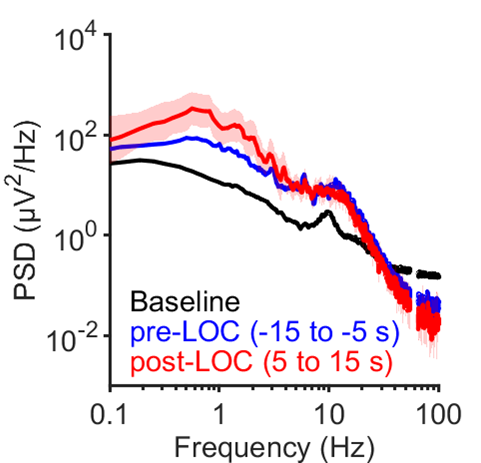
\includegraphics[width=48mm]{Figures/Discussion/delta_rhythms.png}
\vspace{-9pt}
\caption{\captiontitle{High resolution spectra.} n=14. Shading: 95\% confidence interval. LOC: loss of consciousness.} \label{fig:delta_resolution}
\end{wrapfigure}

An analysis that was not included in the paper looked at the group-averaged spectra before and after loss of consciousness at a frequency resolution of \qty{0.1}{\hertz}. With the above caveats to this analysis in mind, these plots did seem to suggest a narrowband increase in the delta range (\autoref{fig:delta_resolution}). However, this observation was not reflected in the individual spectra for each patient --- likely due to poor signal-to-noise ratio for the reasons mentioned above –-- making parameterization impossible. We therefore did not attempt to quantitatively separate the relative contributions of aperiodic and periodic neural activity at low frequencies.

\subsection{Simplified recurrent connections}
In our results in \autoref{sec:natcomms}, recurrent connections were only explicitly modelled between excitatory neurons. The idea was that the inhibitory connections were implicit in the branching number because inhibition plays the role of determining whether a neuron will fire in response to an incoming spike. The reason for this simplification was that it allowed us to control the effective branching number of the network with a single parameter, while also independently specifying the firing rates and E:I ratio of the network. Because of the role of E:I balance in determining network criticality \cite{Lombardi2017}, it was suggested by a reviewer to replicate these results with an E-I network that explicitly models inhibitory connections. 

Notably, it was recently shown theoretically how a network of E-I neurons can be tuned from the asynchronous state to criticality \cite{Li2020}. Performing this tuning would have been necessary to calculate the effect of criticality in an E-I network on dipole synchrony and the spectral trend. However, such simulations were intractable within the scope of our study for several reasons. First, Li and Shrew \cite{Li2020} show how criticality can be tuned in a randomly connected network. The purpose of our simulations were to calculate the effects of network criticality on dipole synchrony and a randomly connected network can never produce dipole synchrony. Unfortunately, imposing a non-random topology on the network violated the assumption of Li and Shrew's theoretical results \cite{Li2020} and the dynamics of the network could no longer be easily tuned. 

Secondly, it was important for our purposes that the firing rates and E:I ratio of the network stay constant so as to isolate the contributions of the dynamics to the dipole synchrony and the resulting power spectra. Unfortunately, changing the branching number of the E-I network using the results of Li and Shew \cite{Li2020} alters the firing rates of excitatory and inhibitory cells. Specifying the E:I balance and effective branching number independently, while also maintaining constant firing rates would be required to properly compare the effects of criticality on the spectral trend. However, solving this problem was not trivial and we therefore stayed with the simplified branching network with enslaved inhibitory neurons.

\begin{figure}[t]
\centering
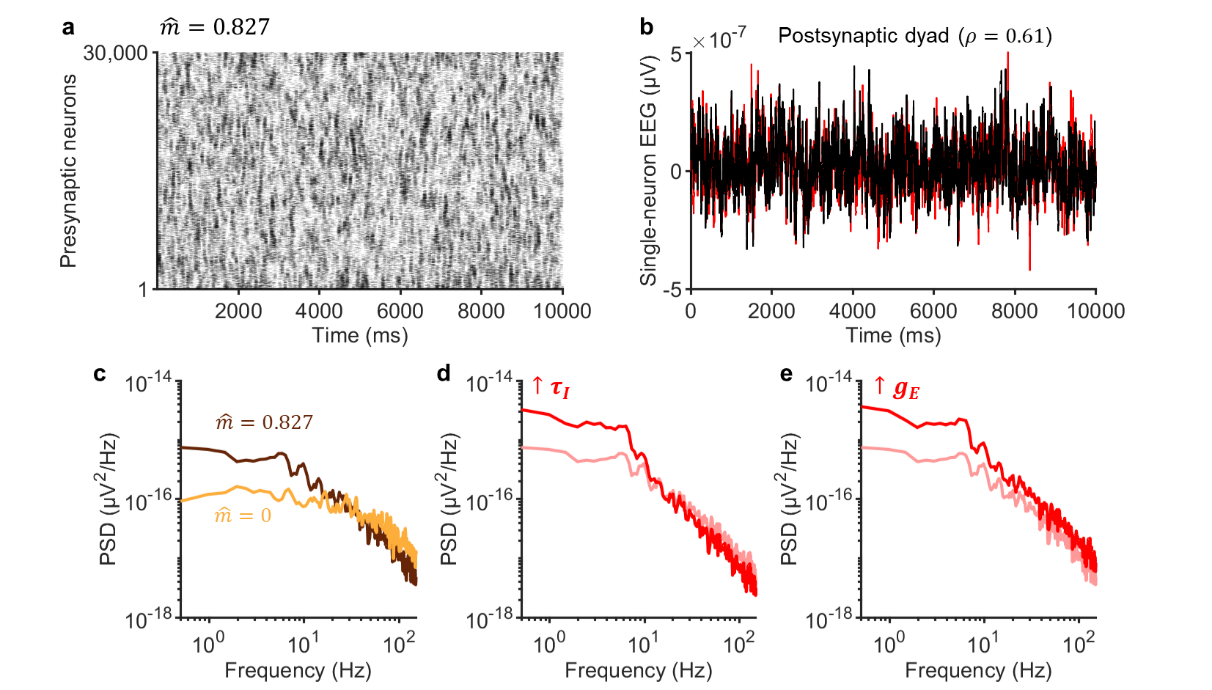
\includegraphics[width=14cm]{Figures/Discussion/subcritical_network.png}
\vspace{-1em}
\caption{\captiontitle{E-I network near criticality generates dipole synchrony.}
\textbf{a} Raster plot of E-I network with 30,000 neurons, with each neuron connected to 2\% of its neighbours. Neurons were embedded in plane with periodic boundary conditions and the probability of connection was proportional to $e^{-d_{ij}}$, where $d_{ij}$ is the pairwise distance. The effective branching number was calculated at each time point as the number of spikes that were transferred from the previous time point. Connections weights were tuned to roughly elicit activity with subcritical dynamics ($\hat{m}\approx0.83$).
\textbf{b} The presynaptic network was projected onto two postsynaptic neurons. Simulated single-neuron EEG signals exhibited correlation of 0.61. 
\textbf{c} Power spectrum of single-neuron EEG elicited by the E-I network (dark brown) compared to the same network with all internal connections severed, i.e., a branching number of zero (light brown).
\textbf{d} Unitary spectrum of E-I network before (light red) and after (red) an increase $\tau_I$, the deactivation kinetics of GABA receptors. 
\textbf{e} Same as panel d, but with an increase in parameter $g_E$, the maximal conductance of AMPA receptors.}
\label{fig:EI_crit}
\vspace{-1em}
\end{figure}

At the request of the reviewer, we did simulate a presynaptic network using an E-I model with a planar topology, i.e., the same topology used for our branching network. Because of the difficulty in tuning the network's level of criticality, we examined a single parameterization that roughly placed the network in a subcritical regime $\hat{m}\approx0.83$ (\autoref{fig:EI_crit}a). This network elicited dipole synchrony (\autoref{fig:EI_crit}b), and changing biophysical parameters produced similar changes to those observed with the branching model used in the \autoref{sec:natcomms} (\autoref{fig:EI_crit}d, e). Comparing the spectrum to that produced by the model with all internal connection severed (i.e., a branching number forced to be zero) revealed that subcritical activity generated the steeper spectrum, consistent with the effects of changing criticality in the branching model used the \autoref{sec:natcomms}. As expected, changing the branching number also altered the firing rates of excitatory and inhibitory cells, making the interpretation of the comparison made in \autoref{fig:EI_crit}c more difficult than the modelling results used in the final paper (\autoref{fig:figure2.4}). The conclusion from these simulations was that a more complex model of E-I interaction would not be expected to qualitatively change the conclusions of \autoref{sec:natcomms}.

\section{Future directions}

\subsection{Network topology and aperiodic activity}
In order to simplify calculations of ensemble EEG power, all our simulations assumed a homogeneous connectivity across the brain. As mentioned in the discussion of \autoref{sec:apEEG}, going beyond this simplified homogeneous model would be interesting for modelling the contribution of action potentials to various EEG oscillations. For the synaptic component of the EEG, modelling more global connectivity patterns would also be of interest, because the spectral trend has been shown to depend on brain region \cite{He2010,Gao2020}. A recent study simulated brain-wide critical network dynamics using a graph theoretical framework \cite{LEE2019}. The authors defined graph edges with anatomical brain connectivity data and node dynamics with simple Kuramoto models, before feeding the output into a forward EEG model to simulate the dynamics of different EEG electrodes. This allowed the authors to investigate how differences in network criticality alter the statistical relations among EEG electrodes, specifically their phase lag entropy, which was then compared to EEG data collected during various states of consciousness  \cite{LEE2019}. In future work, it would be interesting to adopt a similar modelling framework, but adapted to more biophysical source current models such as the single-neuron dipole approach used here, in order to investigate variation in the EEG spectral trend across the scalp.

\subsection{Loss and recovery of consciousness from GABAergic agents}
In addition to propofol, many anesthetics and sedatives act as GABA\textsubscript{A} receptor modulators, including isoflurane, sevoflurane, etomidate, methohexital, and thiopental \cite{Brohan2017}. Whether these drugs share a common mechanism to induce loss of consciousness is still unclear. Notably, these drugs do not necessarily exhibit the same EEG signatures. For example, sevoflurane was found to produce more EEG power across a broad range of frequencies compared to propfool \cite{Akeju2014}. Even though all these drugs modulate GABA\textsubscript{A} receptors, subtle differences in their effects on channel gating may lead to distinct broadband changes in the EEG signal. An interesting future direction would be to compare the broadband changes induced by each of these GABAergic agents and to reexamine the spectral changes associated with loss of consciousness with and without spectral detrending. Such studies could help identify commonalities among agents that induce loss of consciousness and lead to deeper insights into the neural basis of consciousness.

Previous work has investigated the EEG signatures of both loss and recovery of consciousness from propofol \cite{Purdon2013}. In this previous study, arousal levels were evaluated by asking subjects to respond to an auditory stimulus with a button press every \qty{4}{\second}. The decline and subsequent resurgence in the probability of responding to the stimuli was then used to defined moments of loss and recovery of consciousness. This paradigm revealed correlated increases in delta and alpha oscillations upon losing consciousness and a symmetric decrease upon regaining consciousness  \cite{Purdon2013}. Our findings deviate from this study as we observed that, after spectral detrending, the appearance of alpha power preceded that of delta power upon losing consciousness. This observation raises the question of whether spectral detrending may reveal differences in the time course of alpha and delta oscillations upon recovery of consciousness as well. In addition to delineating the functional consequences of propofol-induced alpha and delta oscillations, such investigations would help further characterize the phenomenon of ``neural inertia'', a form of hysteresis whereby regaining consciousness requires drug concentration to decrease well below the level that produced unconsciousness \cite{Kim2018, Warnaby2017, Voss2012, Joiner2013, Friedman2010, Steyn-Ross2004} and which has been specifically related to hysteresis in delta power \cite{Warnaby2017}.

\subsection{Investigating currents from other ligand-gated channels}
In our modelling work, fast synaptic and voltage-gated currents were seemingly sufficient to capture almost all the spectral features of EEG above \qty{1}{\hertz}. However, infraslow EEG recordings illustrate interesting features of the spectral trend at frequencies below \qty{1}{\hertz} (e.g., \autoref{fig:phenomenology}B). In this frequency range, the contributions of all the currents studied here have a predominantly flat frequency response. It is possible that the kinetics of slower currents, such as leak currents, NMDA currents, or even currents induced by metabotropic receptors, such as GABA\textsubscript{B} receptor, could impart filtering effects at these lower frequencies. Currents gated by neuromodulators were not studied at all in this thesis and may be particularly interesting to explore because many neuromodulators operate through volume transmission, where neuromodulator is released into the extracellular space across a wide volume of tissue \cite{Ozcete2024}. This could potentially synchronize the activation of many currents and generate low frequency EEG signals. Biophysical simulations that incorporate the density of neuromodulator receptors with the dynamics and amplitudes of the resulting currents could reveal whether these mechanisms are expected to generate detectable EEG signals. With the increasing prevalence of genetically-encoded fluorescence sensors for myriad neurotransmitters --- including glutamate \cite{Marvin2013}, GABA \cite{Marvin2019}, acetylcholine \cite{Jing2018}, serotonin \cite{Wan2021}, and more --- transient changes in ligand concentration could be measured while simultaneously recording EEG signals in mice \cite{Kim2024,Teng2023}. Empirical associations could then be made between EEG features and specific ligands, similarly to how, sixty years ago, in vivo whole cell recording were used to statistically relate subthreshold currents with EEG \cite{KLEE1965}.

\subsection{Nonparametric data-driven spectral analysis}
The results from this thesis suggest that many different aspects of neuronal physiology converge to shape EEG spectra, including firing rates, average membrane potential, dendritic filtering, synapse kinetics, and more. While the spectral exponent could not be used to distinguish all these mechanisms in our simulations, there could be deeper information about the underlying mechanisms when changes across the entire spectral trend are examined. As a future direction, it would be interesting to train machine learning classifiers on simulated EEG spectra to determine how much information about the underlying mechanistic changes are present in the final EEG spectrum. The results from such work could eventually be used to develop a nonparameteric analysis tool to infer neurophysiological changes from EEG in a purely data-driven framework. Such a tool would be a significant improvement over the current state of fitting the slope of the EEG spectrum, which our findings indicate does not have a unique interpretation. Critically, if successful, such a tool could help determine whether broadband changes in an EEG spectrum need to be rectified and if so how this rectification should be performed.

\section{Concluding remarks}
The ultimate goal of elucidating the neurophysiological basis of EEG is to gain deeper mechanistic insight into brain function and dysfunction. The work in this thesis demonstrates that EEG offers information about the brain beyond the dynamics of its oscillating neural assemblies. Through analysis of its broadband spectral trend, EEG discloses information on the molecular and cellular properties that together shape the generation of the brain's electric fields. While continued investigations work to establish a complete understanding of this physiology, the next challenge will be extracting this information within a data-drive framework. These tools will certainly be useful for interpreting neurological changes induced by GABA receptor modulators, which in addition to anesthetics notably include barbiturates and benzodiazepines. Mining what was once considered background noise for physiological information thus promises new avenues of research into pharmacologically-induced states of consciousness as well as drug therapies for disorders such as epilepsy. Despite its century of use, EEG still holds many secrets waiting to be explored.